\documentclass{beamer}
\usepackage[utf8]{inputenc}

\usetheme{Madrid}
\usecolortheme{default}
\usepackage{amsmath,amssymb,amsfonts,amsthm}
\usepackage{txfonts}
\usepackage{tkz-euclide}
\usepackage{listings}
\usepackage{adjustbox}
\usepackage{array}
\usepackage{tabularx}
\usepackage{gvv}
\usepackage{lmodern}
\usepackage{circuitikz}
\usepackage{tikz}
\usepackage{graphicx}

\setbeamertemplate{page number in head/foot}[totalframenumber]

\usepackage{tcolorbox}
\tcbuselibrary{minted,breakable,xparse,skins}



\definecolor{bg}{gray}{0.95}
\DeclareTCBListing{mintedbox}{O{}m!O{}}{%
	breakable=true,
	listing engine=minted,
	listing only,
	minted language=#2,
	minted style=default,
	minted options={%
		linenos,
		gobble=0,
		breaklines=true,
		breakafter=,,
		fontsize=\small,
		numbersep=8pt,
		#1},
	boxsep=0pt,
	left skip=0pt,
	right skip=0pt,
	left=25pt,
	right=0pt,
	top=3pt,
	bottom=3pt,
	arc=5pt,
	leftrule=0pt,
	rightrule=0pt,
	bottomrule=2pt,
	toprule=2pt,
	colback=bg,
	colframe=orange!70,
	enhanced,
	overlay={%
		\begin{tcbclipinterior}
			\fill[orange!20!white] (frame.south west) rectangle ([xshift=20pt]frame.north west);
	\end{tcbclipinterior}},
	#3,
}
\lstset{
	language=C,
	basicstyle=\ttfamily\small,
	keywordstyle=\color{blue},
	stringstyle=\color{orange},
	commentstyle=\color{green!60!black},
	numbers=left,
	numberstyle=\tiny\color{gray},
	breaklines=true,
	showstringspaces=false,
}
%------------------------------------------------------------
%This block of code defines the information to appear in the
%Title page
\title %optional
{4.7.39}

%\subtitle{A short story}

\author % (optional)
{Nipun Dasari - EE25BTECH11042}



\begin{document}
	
	\frame{\titlepage}
	\begin{frame}{Question}
		The distance of the point P(2, 3) from the x-axis is?
	\end{frame}
	
	
	\begin{frame}{Theoretical Solution}
		Consider the general line equation where 
	\begin{align}
		\vec{n}^\top\vec{x} = c
	\end{align}
	Using the fact that all y-coordinates of x axis are zero
	
	\begin{align}
		\vec{n} = \begin{myvec} { 0\\ 1} \end{myvec} \text{ and } c=0 \label{1}
	\end{align}
	
	The distance between a $\vec{p}$ to its foot of perpendicular to a line is: 
		
		
	\end{frame}
	\begin{frame}{Theoretical Solution}
		\begin{align}
		\text{Distance} = \frac{|\vec{n}^\top\vec{p}-c|}{\norm{\vec{n}}} \label{2}
	\end{align}
	By \eqref{2} and \eqref{1}:
	\begin{align}
		\text{Distance} = \frac{|\begin{myvec} { 0& 1} \end{myvec}\begin{myvec}{ 2 \\ 3 }\end{myvec}-0|}{1}\\
		= 2\times0 + 3\times1 = 3
	\end{align}
	Therefore, the distance of point P from the x-axis is $3$ units.

\end{frame}
	
	\begin{frame}[fragile]
		\frametitle{C Code- distance }
		
		\begin{lstlisting}
			#include <math.h>
			void calculate_distance_from_xaxis(
			double* input_P,        // Pointer to a 2-element array [Px, Py]
			double* output_distance // Pointer to a 1-element array to be filled
			) {
				// Unpack the y-coordinate from the input point
				double Py = input_P[1];
				
				// The distance is the absolute value of the y-coordinate
				double distance = fabs(Py);
				
				// Fill the output array with the calculated distance
				output_distance[0] = distance;
			}
		\end{lstlisting}
	\end{frame}
	
	\begin{frame}[fragile]
		\frametitle{Python Code using shared output}
		\begin{lstlisting}
		import ctypes
		import numpy as np
		import matplotlib.pyplot as plt
		
		# --- Step 1: Load the shared library ---
		lib = ctypes.CDLL('./4.7.39.so')
		
		# --- Step 2: Define the C function signature using NumPy-aware pointers ---
		calculate_distance = lib.calculate_distance_from_xaxis
		
		# Define the argument types
		calculate_distance.argtypes = [
		np.ctypeslib.ndpointer(dtype=np.double, ndim=1, flags='C_CONTIGUOUS'), # input_P
		np.ctypeslib.ndpointer(dtype=np.double, ndim=1, flags='C_CONTIGUOUS')  # output_distance
		]
		# The function has a 'void' return type in C
		calculate_distance.restype = None
		
		\end{lstlisting}
	\end{frame}
	\begin{frame}[fragile]
		\frametitle{Python Code using shared output}
		\begin{lstlisting}		
		# --- Step 3: Prepare NumPy arrays and call the C function ---
		# Define the point P as a NumPy array
		P = np.array([2.0, 3.0], dtype=np.double)
		
		# Create an empty NumPy array for the C function to fill
		output_data = np.zeros(1, dtype=np.double)
		
		# Call the C function. NumPy arrays are passed directly.
		calculate_distance(P, output_data)
		
		# --- Step 4: Extract the result and plot ---
		# The calculated distance is the first (and only) element in the output array
		distance = output_data[0]
		print(f"Point P Coordinates: ({P[0]}, {P[1]})")
		print(f"Distance from x-axis (calculated by C): {distance:.4f}")
		\end{lstlisting}
	\end{frame}
	\begin{frame}[fragile]
		\frametitle{Python Code using shared output}
		\begin{lstlisting}
			# Setup for plotting
			fig, ax = plt.subplots(figsize=(8, 8))
			ax.set_aspect('equal', adjustable='box')
			ax.grid(True, linestyle=':', alpha=0.7)
			
			# The projection of P onto the x-axis is Q
			Q = np.array([P[0], 0.0])
			
			# Plot the distance line between P and Q
			ax.plot([P[0], Q[0]], [P[1], Q[1]], 'g--', label=f'Distance = {distance:.2f}')
			
			# Plot point P and its projection Q
			ax.plot(P[0], P[1], 'o', markersize=10, color='red', label=f'Point P({P[0]}, {P[1]})')
			ax.text(P[0] + 0.1, P[1] + 0.1, 'P', fontsize=14, fontweight='bold', color='red')
			ax.plot(Q[0], Q[1], 'o', markersize=8, color='blue')
			ax.text(Q[0] + 0.1, Q[1] + 0.1, 'Q', fontsize=14, fontweight='bold', color='blue')
		\end{lstlisting}
	\end{frame}
	\begin{frame}[fragile]
		\frametitle{Python Code using shared output}
		\begin{lstlisting}
			# Axes and Title
			ax.axhline(0, color='black', linewidth=0.8)
			ax.axvline(0, color='black', linewidth=0.8)
			ax.set_xlim(-1, 5)
			ax.set_ylim(-1, 5)
			ax.set_title('Distance of Point P from the x-axis', fontsize=16)
			ax.legend(loc="upper left")
			
			# Save the figure to be used in the LaTeX document
			plt.savefig('distance_plot.png')
			
			plt.show()
		\end{lstlisting}
	\end{frame}
	

	\begin{frame}{Plot by python using shared output from c}
		\begin{center}
			\begin{figure}[H]
				\centering
				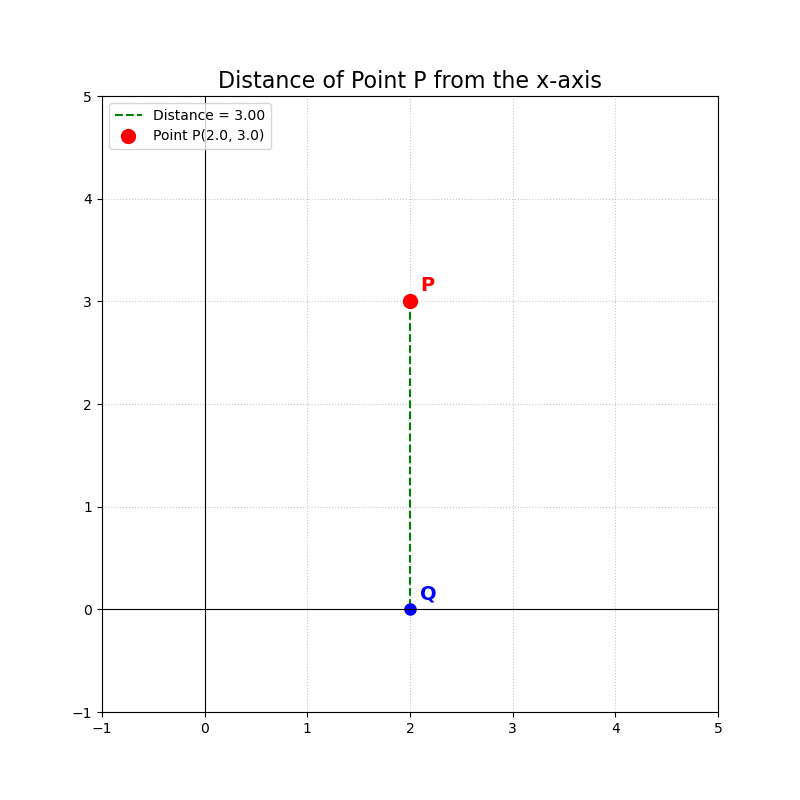
\includegraphics[width = 0.6\columnwidth]{figs/Figure_1.png}
				\caption*{}
				\label{}
			\end{figure}
		\end{center}
	\end{frame}
	\begin{frame}{Plot by python only}
		\begin{center}
			\begin{figure}[H]
				\centering
				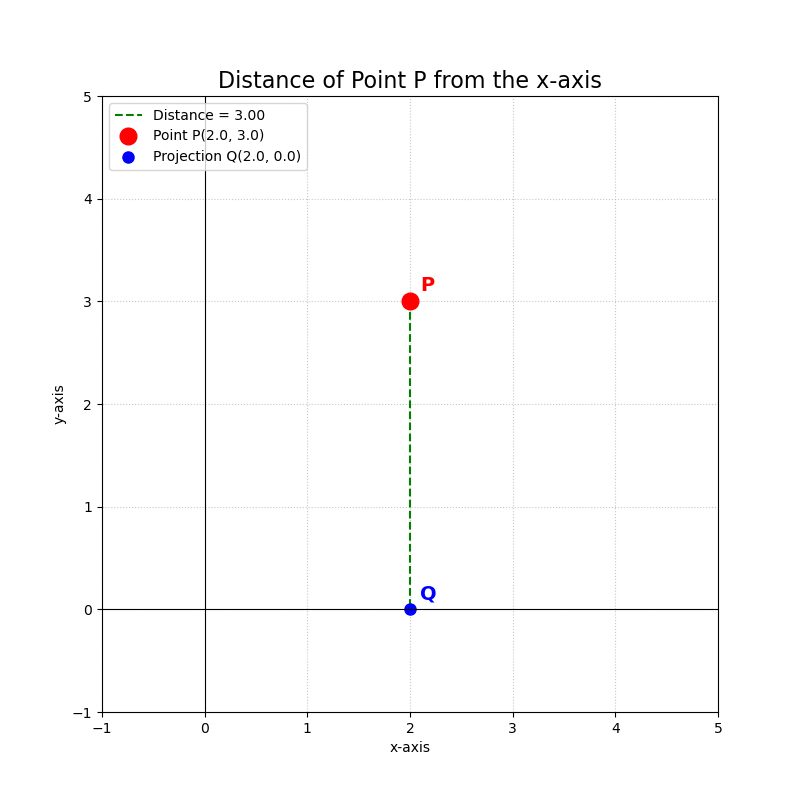
\includegraphics[width = 0.6\columnwidth]{figs/Figure_2.png}
				\caption*{}
				\label{}
			\end{figure}
			
		\end{center}
	\end{frame}
	
\end{document}